\en

\section**{Problem outline}
\label{sec:problem}

Representing 96,3\% of the top one million web servers and 85\% of smartphones worldwide, the Linux kernel is an open-source 
project providing value to billions of people daily. The magnitude that the project has reached over the years makes 
the addition of features, as well as handling bugs and security vulnerabilities, potentially affect a significant 
number of people, demonstrating the importance of maintaining the kernel \citep{linuxdata}.

Maintaining the Linux kernel is a complex task, as the project contains more than 19 million 
lines of code and has more than thirteen thousand contributors along the project's lifespan
\citep{linuxquantity}.
Given the magnitude of the project, it is unrealistic to expect that all contributors 
followed the best programming practices and principles throughout every contribution they made to the project.
It is expected to find a good amount of bad-quality code artifacts in the source code, 
which could result in hindering or compromising the maintenance of this project, as well as the 
addition of new features for it.

Device drivers, as stated by Madieu, are a "piece of software whose aim is to control and manage
a particular hardware device, hence the name device driver"
\citep{driverdef}. 
Device drivers are a major part of the Linux kernel, representing 66 \% of the source code, and 
are responsible for the management of crucial elements such as keyboards, mice, and GPU
\citep{marcelo}. 
The moment the kernel chooses to support new hardware, it is required to make alterations to existent 
device drivers or the creation of new ones, this makes the maintainment of the device drivers 
an important duty of the Linux community.

The AMD Display driver of the Linux kernel is the driver responsible for enabling AMD GPUs to operate 
correctly in desktop Linux environments, which is an important duty, given that AMD GPU represented 19 \% 
of the personal GPU market in 2023  \citep{gpumarket} . 
When we interacted with the maintainers of the AMD Display driver, they shared with us their pain with one 
of the characteristics of bad quality code artifacts, which are duplicated code artifacts, which hinder 
the maintainment of the driver.

Searching for solutions to the AMD Display driver problem with duplicated code artifacts, we were 
able to find tools that gave two code artifacts, infer if they are duplications of each other, and the 
formal literature in the code duplication mainly focused on optimizing the accuracy of these tools in this 
given task. These solutions do not address our problem, as we are not able to give them a codebase and 
they return to us the code duplication in the codebase, and they do not guide us to how to mitigate the code 
duplications after we detected them, requiring us to search for others alternatives.

Given the unsuccessful results of our search in the formal literature, we started to search for solutions in the 
gray literature, but we ended up without success. In the gray literature, the best solutions we found were 
primitive solutions that find every pair of code files that are duplications. 
The code files on the AMD Display driver that 
contain duplicated code normally also have specific code that is only implemented in this file. 
Thus, a solution that finds duplication in a deeper context is necessary to find correct duplications 
in the Linux kernel context.

\section**{Research Design}

The code duplication problem outlined in the Section above cannot be resolved by the solutions 
presented in the formal literature or the gray literature, we intend to propose an approach to 
identify and mitigate the code duplications in the Linux Kernel. For that, we propose a tool capable 
of identifying duplicated functions in the kernel, and we intend to mitigate code duplications in the 
Linux Kernel.

In this research, we expect to extract patterns of software engineers' techniques, such as refactoring methods, 
which we commonly use to mitigate code duplications, thus, serving as guidance to future contributors to 
approach the code duplication problem in the given context. To properly investigate our proposed approach,
we developed our primary research question below to guide our research.

\textbf{RQ1:} How effective is our approach in mitigating duplicate code in the Linux kernel?

Given the complexity of the proposed question, we created a supplementary research question to verify midway 
results, which is related to the performance of our proposed tool in the Linux kernel, the supplementary research question
is defined as:

\textbf{RQ1.1:} How accurate is the proposed tool for detecting duplicate functions?


To address our research question, we do a multiple-method research utilizing different methodologies throughout 
the study. We structured this work into two phases, each with distinct research methods.

In \textbf{Phase I}, we will propose, build, and validate a tool capable 
of identifying code duplications at the function level for the C programming language. We expect this proposed tool 
to identify code duplications in the Linux kernel, as in our preliminary investigation of the code files in the kernel 
is commonly a union of duplicated and nonduplicated functions. To validate the tool, we will do a triangulation of results 
by evaluating our tool in the code duplication databases used in the formal literature and doing an empirical analysis 
in a set of randomly selected codes of the AMD Display driver which our proposed tool claims is a duplication. 
A detailed explication of how we will validate our tool is demonstrated in Chapter \ref{cha:method}.

\begin{figure}
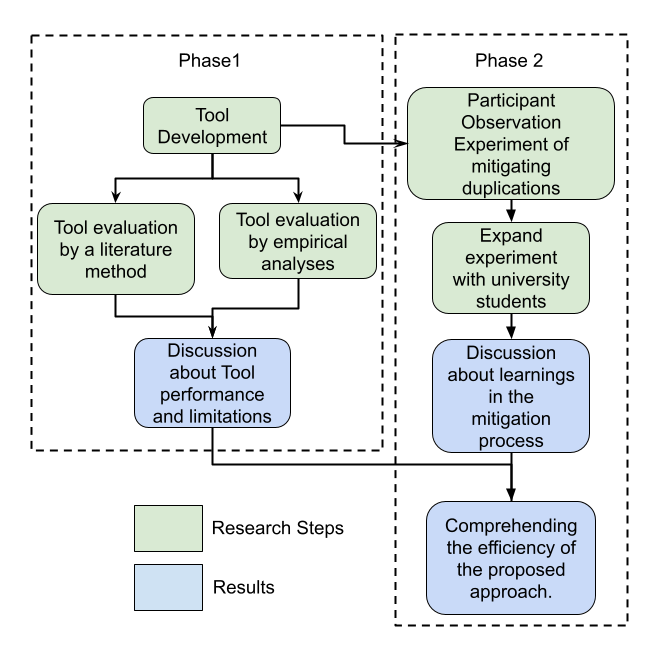
\includegraphics[scale=0.7]{research_design}
\caption{Diagram of the research design.}
\label{fig:reDesign}
\end{figure}

Given the first phase completion, we would have a validated tool to identify code duplications in the Linux kernel 
context and, we can move on to how to mitigate these duplications, which comprehend the second phase of our research.
In \textbf{Phase 2}, we intend to discover ways to mitigate the code duplication detected in the Linux kernel. 
To achieve our objective, we designed an ethnographic approach, which enables us to interact with the Linux community 
to collect artifacts validating or refuting our mitigation.

Figure \ref{fig:reDesign} sumamarizes the research steps proposed in this work.

\section**{Manuscript Structure}

This manuscript consists of five more chapters.
Chapter \ref{cha:back} presents the literature overview for code duplication detection (main definitions, 
current approaches in the literature), a brief description of the Linux kernel, and a review of refactoring methods 
used throughout this research.
Chapter \ref{cha:tool} presents our proposed tool to detect code duplication in the Linux kernel, describing all 
the main components.
Chapter \ref{cha:method} describes the research methods selected to guide our work.
Chapter \ref{cha:eval} shows the results obtained of the research methods to evaluate our proposed tool.
Chapter \ref{cha:results} presents the current research stage and the work plan, with the addition of 
preliminary results obtained.
